%%%%%%%%%%%%%%%%%%%%%%%%%%%%%%%%%%%%%%%%%%%%%%%%%%%%%%%%%%%%%%%%%%%%%%
%%                     Domain
%%%%%%%%%%%%%%%%%%%%%%%%%%%%%%%%%%%%%%%%%%%%%%%%%%%%%%%%%%%%%%%%%%%%%%
\color{red}

\subsection{Glyph: \glyph{Domain}}
\label{sec:domain}

\begin{glyphDescription}

\glyphSboTerm SBO:new

\glyphContainer A domain is represented by a subsection of the carrying \glyph{entity} bordered by two lines 

\glyphLabel A \glyph{domain} is identified by a label placed in an unbordered box containing a string of characters.  The characters can be distributed on several lines to improve readability, although this is not mandatory.  The label box must be attached to the center of the container.  The label may spill outside of the container.

\glyphAux A \glyph{domain} can carry state variables that can add information about its state (\sect{stateVariable}).  A state variable is represented by a rectangle capped with two hemi-circles, with the long axis of this  ``stadium'' placed on the border of the \glyph{domain}'s container, as illustrated in \fig{domain}.  The label of the state variable (which can precise the type of characteristic represented by the state variable, residue type, residue number etc.) is written within the state variable's container. \glyph{Domains} can carry the particular \glyph{state variable} location (\sect{location}). However they cannot carry the particular \glyph{state variable} existence (\sect{existence}), that can only be carried by the main subsection of an \glyph{entity}.

A \glyph{domain} can carry one or several \glyph{units of information} (\sect{unitInfo}). The center of the bounding box of a \glyph{unit of information} is located on the mid-line of the border of the macromolecule.

\end{glyphDescription}

\begin{figure}[H]
  \centering
  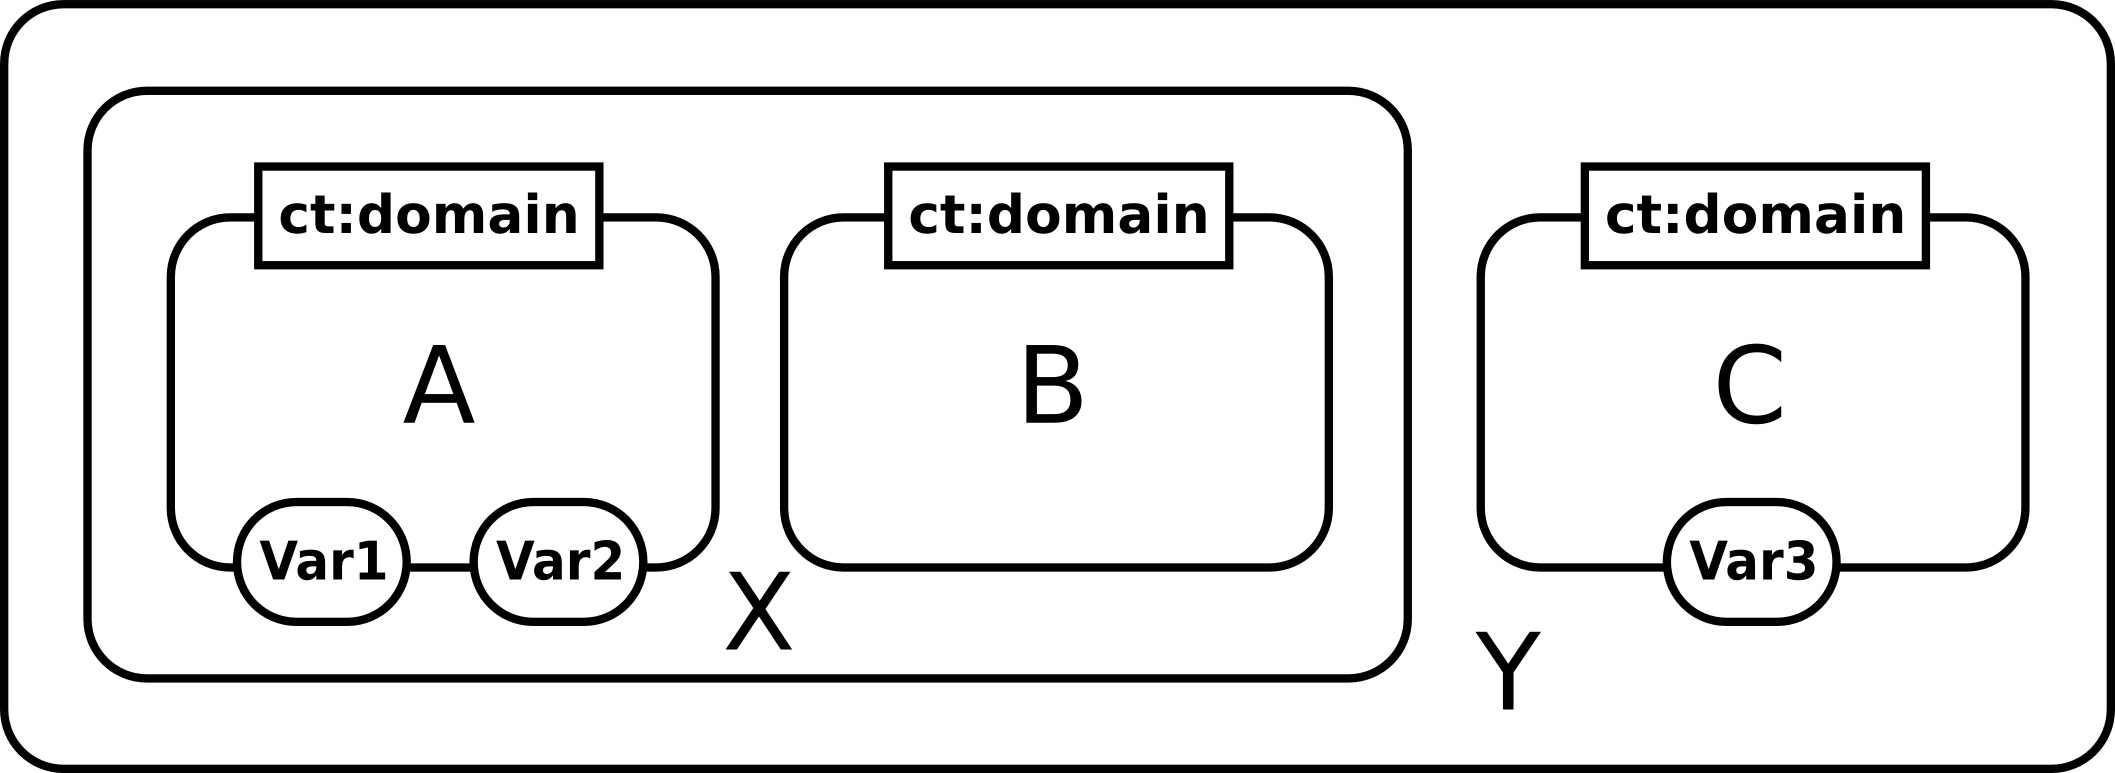
\includegraphics[scale = 0.3]{images/domain}
  \caption{The \ER glyph for \glyph{domain}.}
  \label{fig:domain}
\end{figure}

\begin{figure}[H]
  \centering
  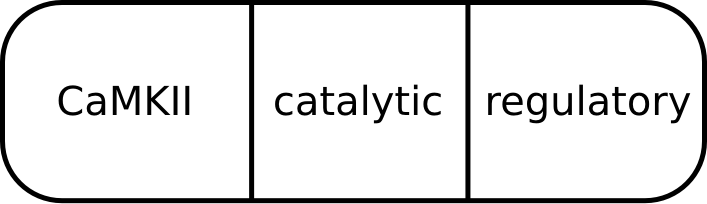
\includegraphics[scale = 0.5]{examples/ex-domain}
  \caption{Examples of \glyph{domains} of the entity CaMKII, representing the catalytic and regulatory portions of the enzyme. The leftward portion of the entity represent the whole entity.}
  \label{fig:ex-domain}
\end{figure}

\normalcolor